% !TEX program = pdflatex
% Statistical Pharmacology via Kakutani Dichotomy X
% Companion computations: code/exp10_ad_tau_abeta_idp_stabilizer.py, code/paper10_compute_tables.py
\documentclass[11pt,reqno]{amsart}

\usepackage[T1]{fontenc}
\usepackage[utf8]{inputenc}
\usepackage{lmodern}
\usepackage[a4paper,margin=27mm]{geometry}
\usepackage{amsmath,amssymb,amsthm,mathtools}
\usepackage{booktabs}
\usepackage{graphicx}
\graphicspath{{./}{../figures/}}
\usepackage{array}
\usepackage[expansion=false]{microtype}
\usepackage{enumitem}
\usepackage{xcolor}
\usepackage[colorlinks=true,linkcolor=blue!60!black,citecolor=blue!60!black,urlcolor=blue!60!black]{hyperref}

\theoremstyle{plain}
\newtheorem{theorem}{Theorem}[section]
\newtheorem{lemma}[theorem]{Lemma}
\newtheorem{proposition}[theorem]{Proposition}
\newtheorem{corollary}[theorem]{Corollary}
\theoremstyle{definition}
\newtheorem{definition}[theorem]{Definition}
\newtheorem{observation}[theorem]{Numerical observation}
\theoremstyle{remark}
\newtheorem{remark}[theorem]{Remark}
\numberwithin{equation}{section}

\newcommand{\Ab}{\mathrm{A}\beta}
\newcommand{\Kt}{K_{\mathrm{tail}}}
\newcommand{\Khot}{K_{\mathrm{hot}}}
\newcommand{\Dt}{D_{\mathrm{tail}}}
\newcommand{\ac}{\alpha_c}
\newcommand{\aeff}{\alpha_{\mathrm{eff}}}
\newcommand{\ath}{\alpha_{\mathrm{th}}}
\newcommand{\kT}{k_{B}T}
\newcommand{\pkg}{\texttt{kakutani\_pharma}}
\newcommand{\lead}{\texttt{KMS-Tau-204}}

\renewcommand{\abstractname}{Summary}
\setlength{\emergencystretch}{3em}
\raggedbottom

% Section 5 is a block of floats; let them pack densely instead of leaving half-empty pages.
\setcounter{topnumber}{4}
\setcounter{bottomnumber}{3}
\setcounter{totalnumber}{6}
\renewcommand{\topfraction}{0.96}
\renewcommand{\bottomfraction}{0.96}
\renewcommand{\textfraction}{0.04}
\renewcommand{\floatpagefraction}{0.70}

\title[Statistical pharmacology via Kakutani dichotomy X]{Statistical Pharmacology via Kakutani Dichotomy X:\\ Blocking Amyloid Nucleation of Intrinsically Disordered Tau and $\Ab_{42}$ Monomers via Tail-Exponent Stabilization, Asymmetric Baseline Cubic Corrections, and Finite-Mode Crossover}

\author[Z. Chen]{Zhengyi Chen}
\address{Guangxi Key Laboratory of Drug Discovery and Optimization, School of Pharmacy, Guilin Medical University, Guilin 541199, P.~R. China}
\email{chenzhengyi@glmc.edu.cn}

\author[R. Chen]{Ruqing Chen}
\address{GUT Geoservice Inc., Montreal, Qu\'ebec, Canada}
\email{ruqing@hotmail.com}

\thanks{DOI: \href{https://doi.org/10.5281/zenodo.23068156}{10.5281/zenodo.23068156}.\newline Sources, code and data:\newline \url{https://github.com/Ruqing1963/kakutani-statistical-pharmacology-X}. Papers I--IX of the series are \cite{ChenChen2026I,ChenChen2026II,ChenChen2026III,ChenChen2026IV,ChenChen2026V,ChenChen2026VI,ChenChen2026VII,ChenChen2026VIII,ChenChen2026IX}, the integrating article is \cite{ChenChen2026S}, and the underlying monograph is \cite{Chen2026}.}
\thanks{This project was supported by the National Natural Science Foundation of China (No.~22464010), the Guangxi Natural Science Foundation of China (No.~2025GXNSFAA069294), and the 2025 Bagui Youth Top Talent Project.}
\date{30 September 2026}

\subjclass[2020]{Primary 92C40, 60G30; Secondary 92C45, 41A58, 65G50, 82B26}
\keywords{Kakutani dichotomy, intrinsically disordered protein, tau, amyloid-beta, amyloid nucleation, critical exponent, Hellinger distance, catastrophic cancellation, Alzheimer's disease}

\begin{document}

\begin{abstract}
Papers~VII--IX worked with folded proteins and covariance. This one works with an intrinsically disordered protein, where there is no pocket to dock into and the only structure is a distribution over contacts. The monomer ensemble is a product measure on $\{\text{coil},\beta\}$; the healthy and pathogenic laws differ by a fixed hot-spot part (the hexapeptides \texttt{VQIINK} and \texttt{VQIVYK} of tau, the central cluster and C-terminus of $\Ab$) and a long-range tail $\epsilon_i = c\,i^{-\alpha}$. By Paper~I the tail sum diverges for $\alpha\le1/2$ and converges above, so the two ensembles are mutually singular below the critical exponent and equivalent above it; hyperphosphorylation lowers $\alpha$ and a kinetic ensemble stabiliser must raise it. The stabiliser acts on $\alpha$ alone, so $\Khot$ is identical in every row and the whole effect is attributable to the tail.
(1)~Proposition~\ref{prop:cubic} extends Paper~I's expansion away from $p_0=1/2$. Away from the symmetric point there is a \emph{cubic} term, $B_1=\tfrac18\left(p_0^{-2}-(1-p_0)^{-2}\right)$, odd about $1/2$ and vanishing there, which is why Paper~I saw only a quartic. At the coil baseline $p_0=0.15$ the measured remainder matches $B_1\epsilon/A_1 = 2.745\,\epsilon$ to $1.7\times10^{-4}$. Corollary~\ref{cor:oc} draws the consequence: corrections to Paper~I's asymptotic constants are $O(c)$, not $O(c^2)$.
(2)~Proposition~\ref{prop:stable} replaces the textbook Hellinger formula, which subtracts two numbers of order one to make a result of order $\epsilon^2$, by an exact rationalised identity with no cancellation. At $\epsilon=10^{-6}$ it is $3.57\times10^{6}$ times more accurate; the textbook form has by then turned round and started to grow.
(3)~Proposition~\ref{prop:twoterm} sums the expansion to $\Kt(\alpha,\infty)=A\zeta(2\alpha)-c^3B_1\zeta(3\alpha)+O(c^4)$ for $\alpha>1/2$, with relative error $O(c^2)$; at the physical $c=0.35$ the cubic over-corrects and the series is not usable, which is stated rather than hidden.
(4)~The doubling estimator of Paper~I recovers $\alpha$ to $0.0094$ at $c=0.35$ and $3.4\times10^{-4}$ at $c=0.01$; the residual bias \emph{is} the cubic term and falls as $c^1$.
(5)~Hyperphosphorylated tau ($\alpha=0.30$) is singular with $t_{1/2}=10.0$\,h; \lead{} ($\aeff=0.72$) is equivalent with $t_{1/2}=3.99\times10^8$\,h, a factor $4.0\times10^7$ bought by the exponent alone.
(6)~$\ac=1/2$ is an $N\to\infty$ statement. At finite $N$ there is a crossover, not a step: $\ath(N)$ rises from $0.1311$ to $0.4676$ over $N=10^2$ to $10^7$, approaching $1/2$ from below. Section~\ref{sec:trap} draws the pharmacological consequence, a \emph{sub-threshold false-positive trap}: a modulator reaching only $\aeff=0.42<1/2$ gives $t_{1/2}=1.81\times10^6$\,h at $N=10^3$ and $9.47$\,h at $N=10^5$, as fast as the untreated ensemble, while \lead{} changes by $5.8\,\%$ over the same range. The exponent a stabiliser must actually reach is $\alpha^\ast=0.5179>\ac$.
The model is a product measure on abstract contact modes, its constants are calibrated on one anchor, and \lead{} is a point in parameter space, not a compound. Section~\ref{sec:assess} states six limits and five open problems.
\end{abstract}

\maketitle
\enlargethispage{\baselineskip}
\tableofcontents

%%%%%%%%%%%%%%%%%%%%%%%%%%%%%%%%%%%%%%%%%%%%%%%%%%%%%%%%%%%%%%%%%%%%%%%%%%%%%%%
\section{Introduction: a target with no pocket}
\label{sec:intro}

\subsection{What is different about a disordered target}
Papers~VII and~VIII estimated Kakutani indices from molecular-dynamics ensembles of folded proteins, and Paper~IX used the second-order index to design a modulator of $\gamma$-secretase around a well-defined catalytic block. All of that machinery presumes a structure: a covariance matrix has a basis, and a pocket has a shape.

Tau and the $\Ab_{42}$ monomer have neither. In solution they are intrinsically disordered: there is no fixed three-dimensional pocket, no persistent secondary structure, and no single conformation whose occupancy a ligand can raise. What there is, is a \emph{distribution} over transient contacts, and the disease is a change in that distribution. The pharmacological question becomes a question about measures rather than about shapes, and that is exactly the setting Paper~I built.

The endpoint is also different. For $\gamma$-secretase the read-out was a product ratio, a property of the steady state of a processive enzyme \cite{Takami2009}. Here it is nucleation: a first-passage event whose rate depends on whether a nucleation-competent phase exists at all. That is a tail question about an infinite product, which is the mechanism this whole series transports from \cite{Chen2026}.

The therapeutic record for this target class is poor, and poor in a specific way that motivates what follows. Compounds that block the aggregation of short aggregation-prone peptides --- hexapeptides, or truncated constructs --- are not scarce; compounds that do so for full-length tau in cells, or in an organism, are. The usual explanations are pharmacokinetic: permeability, stability, exposure. Section~\ref{sec:trap} offers a different one, which is neither about the molecule nor about its delivery, and which the model produces without being asked.

\subsection{Why a product measure}
The modelling decision that carries everything else is to describe the monomer ensemble as a product measure over \emph{contact modes} rather than over coordinates. Three things recommend it.

First, it is what an intrinsically disordered chain gives you. There is no mean structure to expand around, so a covariance matrix has no privileged basis; what is measurable, by paramagnetic relaxation enhancement or by single-molecule F\"orster transfer, is the probability that a particular pair of positions is in contact. A distribution over contacts is the natural state variable.

Second, it is the object Kakutani's theorem speaks about. The theorem \cite{Kakutani1948} says that two infinite product measures are either equivalent or mutually singular, never anything between, and that the alternative is decided by whether $\sum_i h_i$ converges. Nothing in the statement requires the factors to be coordinates; they may be any independent features. Choosing contact modes as the factors is therefore not an approximation to a more honest model, it is a choice of which independence to assume --- and Limit~(f) of Section~\ref{sec:assess} says what that assumption costs.

Third, it separates the local from the global in exactly the way the biology does. The hexapeptides are local: six residues whose $\beta$ propensity is a property of their own sequence. The paperclip is global: a pattern of long-range contacts whose statistics decay with contact order. Writing $\epsilon_i$ as a fixed hot-spot part plus a decaying tail is not a convenience, it is the model's one structural commitment, and the decay exponent of that tail is what the whole paper turns on.

\subsection{What the cryo-EM structures fix}
\label{sec:cryoem}
Two structures define the end state that the monomer must be prevented from reaching, and it is worth being precise about what the present model takes from them.

\emph{Tau filaments from Alzheimer's disease} \cite{Fitzpatrick2017}, PDB \texttt{5O3L}, $3.4$--$3.5$\,\AA. Paired helical and straight filaments extracted from patient brain have cores of two identical protofilaments comprising residues $306$--$378$, in a combined cross-$\beta$/$\beta$-helix fold. The ordered core \emph{begins at residue 306}, which is the first residue of the hexapeptide PHF6, \texttt{VQIVYK} ($306$--$311$), the motif whose $\beta$-forming propensity was shown to be necessary for tau assembly into paired helical filaments \cite{vonBergen2000}. That is the structural reason PHF6 is a hot spot in the model below.

\emph{$\Ab_{42}$ fibrils} \cite{Gremer2017}, PDB \texttt{5OQV}, $4.0$\,\AA. Two intertwined protofilaments, with the backbone of all $42$ residues resolved and an LS-shaped subunit topology in which even the N-terminus is part of the cross-$\beta$ structure. The C-terminal residues that $\Ab_{40}$ lacks are ordered in the fibril, which is the structural reason the model gives $\Ab_{42}$ a stronger C-terminal hot spot than $\Ab_{40}$.

\emph{The monomer these come from} is a different object. Solution tau is not extended but folded back on itself in a global hairpin, the ``paperclip'', in which the C-terminus folds over the microtubule-binding repeats and the N-terminus over the C-terminus \cite{Jeganathan2006}. Those are long-range contacts, and they are protective: they shield the aggregation-prone hexapeptides. Pathological phosphorylation loosens them. In the language of this paper, the paperclip \emph{is} the tail, and hyperphosphorylation is a change in its decay exponent.

\emph{What a ligand can do to such a target} is not to occupy a site. Small molecules that act on disordered monomers do so by transient, multi-site, low-affinity association, which shifts the ensemble without ever forming a defined complex: Heller et al.\ characterised this for \texttt{10074-G5} binding the $\Ab_{42}$ monomer, where the effect is an expansion of the conformational entropy of the monomeric state rather than occupancy of a pocket \cite{Heller2020}. The design law of Section~\ref{sec:pharm} is a quantitative version of that idea.

What the model takes from all of this is the topology only: which segments are hot, that they are shielded by long-range contacts, and that a ligand acts on the shielding. No coordinates are used. Limit~(a) of Section~\ref{sec:assess} says this again.

\subsection{Four results}
The paper contributes four things.

First, a \emph{correction to the expansion the series has been using}. Paper~I worked at $p_0=1/2$, where the symmetry $p\mapsto1-p$ kills the odd terms. A disordered coil is not equally likely to be $\beta$, so the application cannot use the symmetric case, and Proposition~\ref{prop:cubic} shows that away from $1/2$ the first correction is \emph{cubic}. Corollary~\ref{cor:oc} draws the practical consequence, which is that finite-amplitude deviations from Paper~I's constants are linear in $c$.

Second, an \emph{exact identity that removes a catastrophic cancellation}. Proposition~\ref{prop:stable} rewrites the squared Hellinger distance so that no cancellation occurs. The gain reaches $3.57\times10^6$ at $\epsilon=10^{-6}$, which matters precisely because the tail modes, where the dichotomy is decided, are the ones with small $\epsilon$.

Third, the \emph{honest form of the critical statement}. $\ac=1/2$ holds as $N\to\infty$. Proposition~\ref{prop:crossover} and Numerical observation~\ref{obs:ath} describe what happens at finite $N$: a crossover whose threshold $\ath(N)$ rises toward $1/2$ from below, never reaching it.

Fourth, a \emph{pharmacological consequence of the third} that we have not seen stated elsewhere. Section~\ref{sec:trap} shows that a modulator which raises the tail exponent without carrying it across $\ac$ buys a finite-size reprieve that looks like complete protection in a short-peptide assay and evaporates at full-length scale. This is a concrete mechanism for a familiar disappointment: aggregation inhibitors that work \emph{in vitro} on short peptides and fail in cells.

\subsection{What this paper does not do}
No structure is used, nothing is docked, no molecular dynamics is run and no molecule is synthesised. The two cryo-EM structures of Section~\ref{sec:cryoem} enter only by fixing which segments are hot and that the solution monomer's long-range contacts are protective; the model's amplitudes are chosen, its barrier law is phenomenological with one fitted constant, and \lead{} is a location in parameter space rather than a compound. The first three results are mathematical statements about the model and are proved; the fourth is a property of the model that we verify numerically and report as such. Section~\ref{sec:assess} states six limits, of which Limit~(f) --- that contact modes are assumed independent --- is the one that could change a conclusion rather than a number.

%%%%%%%%%%%%%%%%%%%%%%%%%%%%%%%%%%%%%%%%%%%%%%%%%%%%%%%%%%%%%%%%%%%%%%%%%%%%%%%
\section{The ensemble model and the expansion away from one half}
\label{sec:model}

\begin{definition}[Product-measure model of a disordered segment]
\label{def:model}
A segment carries a family of \emph{contact modes}, each a Bernoulli variable that is $\beta$ with probability $p$ and coil otherwise. The healthy soluble ensemble $P$ has $p_i=p_0$ for every mode. The pathogenic pre-nucleation ensemble $Q$ has $p_i=p_0+\epsilon_i$, with
\begin{equation}
\label{eq:eps}
\epsilon_i =
\begin{cases}
\epsilon_{\mathrm{hot}}, & i \text{ in a hot spot (a fixed, finite set)},\\[2pt]
c\,i^{-\alpha}, & i = 1,\dots,N \text{ in the long-range tail}.
\end{cases}
\end{equation}
Throughout $p_0=0.15$, $c=0.35$ and $N=1000$. The hot spots are the hexapeptides PHF6$^\ast$ \texttt{VQIINK} and PHF6 \texttt{VQIVYK} for tau, and the central hydrophobic cluster \texttt{KLVFFA} with the C-terminal segment for $\Ab$; their excesses are listed in Table~\ref{tab:peptides}.
\end{definition}

The index and the affinity are those of Paper~I,
\begin{equation}
\label{eq:index}
h_i = 2\Bigl(1-\sqrt{p_iq_i}-\sqrt{(1-p_i)(1-q_i)}\Bigr),
\qquad K_N = \sum_{i\le N} h_i,
\qquad \Pi_N = \prod_{i\le N}\Bigl(1-\tfrac{h_i}{2}\Bigr),
\end{equation}
and they split additively as $K_N=\Khot+\Kt(\alpha,N)$, with $\Khot$ independent of $\alpha$.

\subsection{An identity without cancellation}

\begin{proposition}[Rationalised Hellinger distance]
\label{prop:stable}
For $p,q\in(0,1)$,
\begin{equation}
\label{eq:stable}
h(p,q) = (p-q)^2\left[\frac{1}{\bigl(\sqrt{p}+\sqrt{q}\bigr)^{2}}+\frac{1}{\bigl(\sqrt{1-p}+\sqrt{1-q}\bigr)^{2}}\right].
\end{equation}
\end{proposition}

\begin{proof}
Expand the two squares $(\sqrt p-\sqrt q)^2 = p+q-2\sqrt{pq}$ and $(\sqrt{1-p}-\sqrt{1-q})^2 = (1-p)+(1-q)-2\sqrt{(1-p)(1-q)}$ and add; the linear terms sum to $2$, giving $(\sqrt p-\sqrt q)^2+(\sqrt{1-p}-\sqrt{1-q})^2 = h(p,q)$ as in \eqref{eq:index}. Rationalise each difference of square roots, $\sqrt p-\sqrt q = (p-q)/(\sqrt p+\sqrt q)$, and factor out $(p-q)^2$.
\end{proof}

\begin{remark}
\label{rem:cancel}
The two sides are algebraically identical and numerically are not. In \eqref{eq:index} two quantities of order one are subtracted to produce a result of order $\epsilon^2$, so about $2\log_{10}(1/\epsilon)$ digits are lost; in \eqref{eq:stable} nothing is subtracted except $p-q$, which is the input. Table~\ref{tab:identity} measures both against the series of Proposition~\ref{prop:cubic}: the two agree at $\epsilon=10^{-3}$, and by $\epsilon=10^{-6}$ the rationalised form is $3.57\times10^{6}$ times closer, because the textbook form has stopped converging and begun to diverge. This is not a fastidious point. The modes that decide the dichotomy are the far tail, where $\epsilon_i$ is smallest.
\end{remark}

\subsection{The cubic term}

\begin{proposition}[Expansion at an asymmetric baseline]
\label{prop:cubic}
For fixed $p_0\in(0,1)$ and $\epsilon\to0$,
\begin{equation}
\label{eq:cubic}
h(p_0,p_0+\epsilon) = A_1(p_0)\,\epsilon^2 - B_1(p_0)\,\epsilon^3 + O(\epsilon^4),
\end{equation}
where
\begin{equation}
\label{eq:coeffs}
A_1(p_0) = \frac{1}{4p_0(1-p_0)},
\qquad
B_1(p_0) = \frac{1}{8}\left(\frac{1}{p_0^2}-\frac{1}{(1-p_0)^2}\right).
\end{equation}
Moreover $B_1(1-p_0)=-B_1(p_0)$, so $B_1$ vanishes if and only if $p_0=1/2$, where the expansion reduces to Paper~I's $h(\delta)=\delta^2+\tfrac54\delta^4+O(\delta^6)$.
\end{proposition}

\begin{proof}
Write $\sqrt{p_0(p_0+\epsilon)} = p_0\sqrt{1+\epsilon/p_0}$ and $\sqrt{(1-p_0)(1-p_0-\epsilon)} = (1-p_0)\sqrt{1-\epsilon/(1-p_0)}$, and expand both by the binomial series:
\begin{align*}
p_0\sqrt{1+\tfrac{\epsilon}{p_0}} &= p_0 + \tfrac{\epsilon}{2} - \tfrac{\epsilon^2}{8p_0} + \tfrac{\epsilon^3}{16p_0^2} + O(\epsilon^4),\\
(1-p_0)\sqrt{1-\tfrac{\epsilon}{1-p_0}} &= (1-p_0) - \tfrac{\epsilon}{2} - \tfrac{\epsilon^2}{8(1-p_0)} - \tfrac{\epsilon^3}{16(1-p_0)^2} + O(\epsilon^4).
\end{align*}
The terms in $\epsilon$ cancel. Adding and substituting into $h = 2(1-\text{sum})$ gives
\[
h = \frac{\epsilon^2}{4}\left(\frac{1}{p_0}+\frac{1}{1-p_0}\right) - \frac{\epsilon^3}{8}\left(\frac{1}{p_0^2}-\frac{1}{(1-p_0)^2}\right)+O(\epsilon^4),
\]
and $\tfrac14(p_0^{-1}+(1-p_0)^{-1}) = \tfrac14\cdot\tfrac{1}{p_0(1-p_0)}$, which is $A_1$. Replacing $p_0$ by $1-p_0$ in $B_1$ exchanges the two reciprocals and reverses the sign, so $B_1$ is odd about $1/2$ and vanishes there; the symmetry $p\mapsto1-p$ also kills every odd term, leaving the quartic as the first correction, which is Paper~I's case.
\end{proof}

At the coil baseline $p_0=0.15$ this gives $A_1=1.9607843$ and $B_1=5.3825452$, so the relative error of the quadratic term alone is $B_1\epsilon/A_1 = 2.745098\,\epsilon$. Table~\ref{tab:cubic} measures it: at $\epsilon=10^{-4}$ the ratio of measured to predicted remainder is $0.99984$.

\begin{corollary}[Why the deviations are linear in the amplitude]
\label{cor:oc}
Along the tail $\epsilon_i = c\,i^{-\alpha}$, the relative size of the cubic term is $B_1\epsilon_i/A_1$, which is proportional to $c$. Hence every quantity built from the tail inherits an $O(c)$ relative correction to its quadratic-order prediction, not the $O(c^2)$ that holds at $p_0=1/2$. In particular the doubling estimator's bias is $O(c)$, which Table~\ref{tab:trichotomy} and Section~\ref{sec:estimator} confirm.
\end{corollary}

\subsection{The convergent side in closed form}

\begin{proposition}[Two-term formula]
\label{prop:twoterm}
For $\alpha>1/2$,
\begin{equation}
\label{eq:twoterm}
\Kt(\alpha,\infty) = A\,\zeta(2\alpha) - c^3B_1\,\zeta(3\alpha) + O(c^4),
\qquad A = c^2A_1,
\end{equation}
and the relative error of the two-term truncation is $O(c^2)$.
\end{proposition}

\begin{proof}
Substitute $\epsilon_i=c\,i^{-\alpha}$ into \eqref{eq:cubic} and sum. The quadratic terms give $A_1c^2\sum_i i^{-2\alpha}=A\zeta(2\alpha)$, convergent for $\alpha>1/2$; the cubic terms give $-B_1c^3\sum_i i^{-3\alpha}=-c^3B_1\zeta(3\alpha)$, convergent for $\alpha>1/3$; the remainder is $\sum_i O(c^4i^{-4\alpha})=O(c^4)$, convergent for $\alpha>1/4$. Dividing the $O(c^4)$ remainder by the leading $O(c^2)$ term gives the relative statement.
\end{proof}

Table~\ref{tab:twoterm} tests this, and the outcome deserves to be stated plainly rather than buried. The two-term formula is a genuine improvement for $c\lesssim0.1$: at $\alpha=0.72$, $c=0.03$ its relative error is $4.2\times10^{-3}$ against $4.1\times10^{-2}$ for the one-term formula, a factor ten. At the \emph{physical} amplitude $c=0.35$ it is worse than useless: the one-term formula is $31\,\%$ high and the two-term formula is $35\,\%$ low, because the cubic correction over-shoots. The asymptotic series in $c$ is simply not usable at $c=0.35$, and nothing downstream in this paper relies on it. What the paper uses is the \emph{exponent}, which Section~\ref{sec:estimator} shows is recovered accurately even there.

%%%%%%%%%%%%%%%%%%%%%%%%%%%%%%%%%%%%%%%%%%%%%%%%%%%%%%%%%%%%%%%%%%%%%%%%%%%%%%%
\section{The trichotomy, the estimator, and the finite-mode crossover}
\label{sec:trichotomy}

\subsection{The three regimes}
Paper~I, Theorem~3.1, gives the trichotomy: $\Kt(\alpha,N)$ grows as $N^{1-2\alpha}$ for $\alpha<1/2$, as $A\ln N$ at $\alpha=1/2$, and converges for $\alpha>1/2$. By Kakutani's theorem the product measures are mutually singular in the first two cases and equivalent in the third, and $\Pi_N\to0$ exactly when $K_N\to\infty$. Table~\ref{tab:trichotomy} and panels~B and~C of Figure~\ref{fig:main} show both sides of that equivalence over five decades of $N$: at $\alpha=0.25$, $\Pi_{10^5}=6.7\times10^{-31}$, while at $\alpha=0.85$ it sits at $0.834$ and is still falling only in the sixth decimal.

The pharmacological reading is the one the rest of the paper uses. Below $\ac$ the pathogenic ensemble is a distinct phase: a nucleus formed from it is not a fluctuation of the healthy ensemble and does not dissolve back. Above $\ac$ it is a fluctuation, and it does.

\begin{remark}[What the dichotomy does and does not assert]
\label{rem:dichotomy}
It is worth being exact about the content of the trichotomy, because it is easy to over-read. Kakutani's theorem is a statement about two \emph{infinite} product measures. It says that the set of configurations on which they disagree is either negligible for both or carries all the mass of one and none of the other, and that $\sum_ih_i$ decides which. It does not say that anything happens suddenly as a physical parameter is varied, and it does not say that a finite system exhibits two phases.

What a finite system has is a partial sum. $K_N$ is continuous in $\alpha$ for every $N$, and so is every observable built from it. The dichotomy is visible only in how $K_N$ behaves as $N$ grows, which is why the estimator of Section~\ref{sec:estimator} measures a \emph{slope} rather than a value, and why Section~\ref{sec:trap} is about system size rather than about a critical point. Proposition~\ref{prop:crossover} is the bridge: it converts an asymptotic statement about $\alpha$ into a bound that holds at every finite $N$, which is the only form in which the dichotomy can be used to make a design claim.
\end{remark}

\subsection{The affinity as an order parameter}
Kakutani's criterion is usually stated for the sum, but the quantity with a direct reading is the product. The two are tied together quantitatively, and it is worth recording how tightly, because the affinity is what a measurement of ensemble overlap would report.

\begin{proposition}[Two-sided bound]
\label{prop:affinity}
Let $h_i\in[0,2)$ with $h_{\max}=\sup_i h_i<2$, and let $K_N=\sum_{i\le N}h_i$, $\Pi_N=\prod_{i\le N}(1-h_i/2)$. Then
\begin{equation}
\label{eq:affbound}
\exp\!\left(-\frac{K_N}{2}\cdot\frac{1}{1-h_{\max}/2}\right) \;\le\; \Pi_N \;\le\; \exp\!\left(-\frac{K_N}{2}\right).
\end{equation}
In particular $\Pi_N\to0$ if and only if $K_N\to\infty$, and when $h_{\max}$ is small the two bounds pinch: $\Pi_N = e^{-K_N/2}\bigl(1+O(\sum_ih_i^2)\bigr)$.
\end{proposition}

\begin{proof}
Put $x_i=h_i/2\in[0,1)$. The upper bound is $\log(1-x)\le-x$, valid on $[0,1)$, summed. For the lower bound, on $[0,x_{\max}]$ with $x_{\max}<1$ the function $x\mapsto-\log(1-x)/x$ is increasing, so $-\log(1-x_i)\le x_i\cdot\bigl(-\log(1-x_{\max})/x_{\max}\bigr)$; a cruder but cleaner estimate uses $-\log(1-x)\le x/(1-x)\le x/(1-x_{\max})$ on the same interval, which summed gives $-\log\Pi_N\le K_N/(2(1-h_{\max}/2))$. Exponentiating both bounds gives \eqref{eq:affbound}. Both sides tend to zero exactly when $K_N\to\infty$, which is the equivalence. The refinement follows from $\log(1-x)=-x-x^2/2-O(x^3)$.
\end{proof}

The bound is what panel~C of Figure~\ref{fig:main} shows in logarithmic form. Over the whole tail, $h_{\max}=h_1=0.1484$ at $c=0.35$, so $(1-h_{\max}/2)^{-1}=1.080$ and the two bounds in \eqref{eq:affbound} differ by at most eight per cent in the exponent. At $\alpha=0.25$ and $N=10^5$, $K_N=138.84$ and $e^{-K_N/2}=7.09\times10^{-31}$ against a measured $\Pi_N=6.69\times10^{-31}$, agreeing to $6.0\,\%$; at $\alpha=0.85$, $K_N=0.355$ and the agreement is $0.35\,\%$. So the affinity is, to within a few per cent, the exponential of minus half the index, and the dichotomy is the statement that this exponent is either bounded or not.

\subsection{Reading the exponent off the data}
\label{sec:estimator}
The doubling increment of Paper~I, $\Dt(N)=\Kt(2N)-\Kt(N)$, satisfies $\Dt(N)\sim A\,N^{1-2\alpha}\bigl(2^{1-2\alpha}-1\bigr)/(1-2\alpha)$, so the slope of $\ln\Dt$ against $\ln N$ is $1-2\alpha$ for every $\alpha$, negative above $\ac$, zero exactly at it. Inverting, $\widehat\alpha = (1-\text{slope})/2$. Panel~D of Figure~\ref{fig:main} plots the measured slopes against $1-2\alpha$.

Over the ten exponents of Table~\ref{tab:trichotomy} the worst error is $|\widehat\alpha-\alpha| = 0.0094$, at $\alpha=0.25$ where $\epsilon_1$ is largest. By Corollary~\ref{cor:oc} that bias is the cubic term and must be $O(c)$; reducing $c$ from $0.35$ to $0.03$ reduces the worst error from $9.4\times10^{-3}$ to $9.8\times10^{-4}$, a factor $9.6$ for an amplitude ratio of $11.7$, and to $3.4\times10^{-4}$ at $c=0.01$.

Two features of that number deserve comment. The first is that it is small where it needs to be. The quantity the pharmacology depends on is not $\alpha$ itself but which side of $\ac$ it falls on, and near $\alpha=1/2$ the estimator is at its best: $\widehat\alpha=0.4977$ at $\alpha=0.50$, an error of $2.3\times10^{-3}$. The bias grows away from criticality, in the direction where it does not matter.

The second is that this is a different bias from the one Paper~I identified. Paper~I's Theorem~4.1 gives the bias of a direct regression of $K$ on $N$ in a finite window,
\[
\gamma_{\mathrm{eff}} = \frac{1-2\alpha}{1+(1-2\alpha)\,\zeta(2\alpha)\,N^{2\alpha-1}},
\]
whose source is the pole of $\zeta$ at $2\alpha=1$ and which the doubling increment cancels identically. That cancellation still holds here: the estimator of this paper is Paper~I's, unchanged. What remains after it is a \emph{different} error, coming from the cubic term of Proposition~\ref{prop:cubic}, which Paper~I did not have because it worked at $p_0=1/2$. The two are separable by their scaling: the finite-window bias falls as $N^{2\alpha-1}$ at fixed $c$, the cubic bias falls as $c$ at fixed $N$. Table~\ref{tab:trichotomy} holds $N$ fixed and Section~\ref{sec:model}'s $c$-scan holds $\alpha$ fixed, and the two behave as predicted.

\subsection{\texorpdfstring{The crossover at finite $N$}{The crossover at finite N}}

\begin{proposition}[Boundedness above the critical exponent]
\label{prop:crossover}
Fix a reference half-time $t_{\mathrm{ref}}$ and let $K^\ast$ be the value of $K_N$ at which the barrier law of Section~\ref{sec:pharm} returns $t_{\mathrm{ref}}$. For $\alpha>1/2$ the sum $\Kt(\alpha,N)$ is bounded above by $\Kt(\alpha,\infty)$ uniformly in $N$, so if
\begin{equation}
\label{eq:safe}
\Khot + \Kt(\alpha,\infty) < K^\ast
\end{equation}
then $t_{1/2}>t_{\mathrm{ref}}$ at \emph{every} $N$. Since $\Kt(\cdot,\infty)$ is strictly decreasing, \eqref{eq:safe} defines a threshold $\alpha^\ast$ above which protection is unconditional. For $\alpha<1/2$ no such bound exists: $\Kt(\alpha,N)\to\infty$, so $t_{1/2}\to t_0$ however large $t_{\mathrm{ref}}$ is chosen.
\end{proposition}

\begin{proof}
For $\alpha>1/2$ the terms $h_i$ are positive and summable, so the partial sums increase to their limit and $\Kt(\alpha,N)\le\Kt(\alpha,\infty)$ for all $N$; the barrier is decreasing in $K_N$ and the half-time increasing in the barrier, so the bound on $K_N$ is a bound below on $t_{1/2}$. Monotonicity of $\Kt(\cdot,\infty)$ in $\alpha$ follows term by term. For $\alpha<1/2$ the partial sums diverge, and the barrier is floored at zero.
\end{proof}

With $t_{\mathrm{ref}}=100$\,h the numbers are $K^\ast=7.7518$, $\Khot=1.2035$, hence $\Kt^\ast=6.5483$ and
\[
\alpha^\ast = 0.51789 .
\]
Note that $\alpha^\ast>\ac$ strictly. Crossing the critical exponent is necessary for unconditional protection but not sufficient: between $\ac$ and $\alpha^\ast$ the sum converges, but not to a small enough value.

\begin{observation}[The threshold approaches the critical exponent from below]
\label{obs:ath}
Let $\ath(N)$ solve $t_{1/2}(\alpha;N)=100$\,h. Table~\ref{tab:crossover} gives
\begin{align*}
\ath &= 0.1311,\ 0.3142,\ 0.3899 \quad\text{at } N = 10^2,\,10^3,\,10^4,\\
\ath &= 0.4290,\ 0.4524,\ 0.4676 \quad\text{at } N = 10^5,\,10^6,\,10^7,
\end{align*}
increasing monotonically and remaining below $\ac=1/2$ throughout.
\end{observation}

This is the honest form of the critical statement, and we labour it because the temptation to draw a step function at $\alpha=1/2$ for a thousand-mode system is real. There is no step at finite $N$. What there is, is a family of crossovers that sharpen and migrate toward $\ac$ as the system grows, shown in panel~A of Figure~\ref{fig:kinetics}.

%%%%%%%%%%%%%%%%%%%%%%%%%%%%%%%%%%%%%%%%%%%%%%%%%%%%%%%%%%%%%%%%%%%%%%%%%%%%%%%
\section{Pharmacology: the design law and the trap it implies}
\label{sec:pharm}

\subsection{From the index to a half-time}
Above $\ac$ a nucleus dissolves back; below it, it does not. We take the nucleation barrier to fall linearly in the separation and the ThT trace to be logistic:
\begin{equation}
\label{eq:kinetics}
\frac{\Delta G^{\ddagger}}{\kT} = \Bigl(G_0 - \lambda K_N\Bigr)_{\!+},
\qquad
t_{1/2} = t_0\,e^{\Delta G^{\ddagger}/\kT},
\qquad
F(t) = \bigl[1+e^{-k(t-t_{1/2})}\bigr]^{-1},
\end{equation}
with $G_0=30$, $\lambda=2.513$, $t_0=2.70\times10^{-3}$\,h and $k=0.45\,\mathrm{h}^{-1}$. One constant is fitted: $\lambda$ is chosen so that hyperphosphorylated tau has $t_{1/2}=10$\,h at $N=1000$. Every other half-time in the paper follows from that single anchor. The positive part matters only deep in the singular phase, where a linear barrier law has nothing left to say, and the experiment flags the rows where it binds.

The choice of a linear dependence on $K_N$ deserves a word, since it is the one modelling step in the paper with no argument behind it. What is defensible is the \emph{direction}: the further the pathogenic ensemble is from the healthy one, the more stable a nucleus drawn from it, and the lower the barrier to forming one irreversibly. What is not derived is the functional form. Linearity is the simplest law with that monotonicity and with a finite barrier at $K_N=0$, and it has the property that $t_{1/2}$ is exponential in $K_N$, which is what turns the modest spread of $K_N$ in Table~\ref{tab:states} into the eight decades of half-time that the table reports. A different form would move those decades. It would not move any of the following, none of which involve $\lambda$ or $G_0$: the phase assignment of any state, the value of any exponent, the estimator errors, the ratio $\Kt(\alpha,N)$ takes between two system sizes, or the qualitative collapse of Table~\ref{tab:trap}. Open problem~(4) asks for the form to be derived rather than posited.

\subsection{The design law}
Table~\ref{tab:states} gives the four tau states. Hyperphosphorylation ($\alpha=0.30$) is singular, with $\Kt=7.4637$ and $\Pi_N=1.27\times10^{-2}$; \lead{} ($\aeff=0.72$) is equivalent, with $\Kt=0.5000$ and $\Pi_N=0.4183$; the half-time moves from $10.0$\,h to $3.99\times10^8$\,h, a factor $4.0\times10^{7}$.

The column to watch is $\Khot$. It is $1.2035$ in every row, because the stabiliser is defined to act on the tail exponent and on nothing else. That is not a convenience: it is what makes the experiment a test of the design law rather than a demonstration that adding a second effect helps. A compound that also blunted the hexapeptides would be a different, and easier, proposition.

\subsection{The sub-threshold false-positive trap}
\label{sec:trap}
Proposition~\ref{prop:crossover} has a consequence for screening that we believe deserves to be stated on its own. Consider a weak modulator that raises the tail exponent from $0.30$ to $\aeff=0.42$ --- a real improvement, and still below $\ac$. Table~\ref{tab:trap} follows it to two system sizes:

\begin{center}
\begin{tabular}{@{}l r r r@{}}
\toprule
& $\aeff$ & $t_{1/2}$ at $N=10^3$ & $t_{1/2}$ at $N=10^5$\\
\midrule
untreated & $0.30$ & $10.0$\,h & $2.7\times10^{-3}$\,h\\
weak modulator & $0.42$ & $1.81\times10^{6}$\,h & $9.47$\,h\\
\lead{} & $0.72$ & $3.99\times10^{8}$\,h & $3.77\times10^{8}$\,h\\
\bottomrule
\end{tabular}
\end{center}

At the scale of a short-peptide assay the weak modulator looks like a complete block: $1.8$ million hours, nothing measurable over any experiment. Taken to the scale of a full-length protein or a cellular condensate, the series diverges and the protection collapses to $9.47$\,h --- statistically indistinguishable from the $10.0$\,h of the \emph{untreated} ensemble at the smaller scale. \lead{} changes by a factor $1.058$ over the same range, because above $\ac$ the sum is bounded and Proposition~\ref{prop:crossover} applies.

Panel~B of Figure~\ref{fig:kinetics} makes the point in the form an experimentalist would meet it: the ThT trace of the weak modulator at $N=10^5$ lies on top of the untreated trace.

\begin{remark}
This offers a mechanism for a familiar and expensive pattern: aggregation inhibitors that are convincing on hexapeptide or short-construct assays and disappear in full-length cellular models. In this model the failure is not potency, solubility or delivery. It is that the assay was run at a system size whose crossover threshold $\ath(N)$ happened to sit below the compound's $\aeff$, and the target one wants is not ``raise $\alpha$'' but ``raise $\alpha$ past $\alpha^\ast$''. The prediction is testable and, unusually, cheap to test: run the same compound against constructs of increasing length and look for collapse.
\end{remark}

\subsection{What raising the exponent would mean for a chemist}
\label{sec:chemist}
The design law says: raise $\alpha$ past $\alpha^\ast$. That is a statement about a distribution, and it is fair to ask what kind of molecule could satisfy it.

The tail exponent measures how fast the pathogenic excess in contact probability decays with contact order. Raising it means suppressing the \emph{long}-range part of the excess preferentially over the short-range part. A ligand that bound one site tightly would not do this: it would alter a few modes by a large amount, which changes $\Khot$ and leaves the exponent alone. What does do it is the opposite kind of interaction --- weak, transient, distributed over many positions --- because such an interaction competes with long-range contacts everywhere along the chain and competes most effectively where those contacts are weakest, which is at high contact order.

This is the mode of action that has been characterised for small molecules acting on disordered monomers, where binding is fuzzy and the thermodynamic effect is an expansion of the conformational entropy of the monomeric state rather than the formation of a complex \cite{Heller2020}. The present model gives that picture a quantitative target: not ``shift the ensemble'' but ``raise the decay exponent of the long-range contact excess above $0.518$''. Whether any real ligand does so is not something this paper can determine. What it does determine is that the quantity to measure is a \emph{slope}, and Section~\ref{sec:assess}, open problem~(2), asks what the cheapest experiment is that would measure it.

\subsection{Relation to the four-quadrant classifier}
\label{sec:quadrants}
Paper~IV classified ligands of a folded target in the plane of a pocket-visible perturbation against the second-order index, and the useful class was quadrant~II: invisible to a docking screen, loud in the index. Paper~IX used exactly that plane for $\gamma$-secretase.

The disordered case has an analogous plane, with a different pair of axes: $\Khot$ against $\alpha$. A ligand that blunts the hexapeptides moves along the first axis and is visible to any assay that reports on hexapeptide $\beta$ content; a ligand that raises the tail exponent moves along the second and is visible to none of them, because no local measurement sees a change in a decay exponent. The stabiliser of this paper is deliberately placed on the second axis alone, with $\Khot$ held exactly constant across Table~\ref{tab:states}.

The analogy is not perfect and the difference is instructive. In Paper~IV both coordinates were properties of a single ensemble comparison at fixed system size. Here the second coordinate is a property of how the comparison behaves as the system grows, so it cannot be read off one measurement at all. That is precisely why the trap of Section~\ref{sec:trap} exists, and it has no counterpart in the folded-target papers.

\subsection{\texorpdfstring{$\Ab_{42}$ against $\Ab_{40}$}{Abeta42 against Abeta40}}
\label{sec:abeta}
The two peptides differ by Ile41 and Ala42. Holding the tail exponent equal, the C-terminal hot spot alone gives $\Delta\Khot=0.4274$ and a half-time ratio of $2.93$ ($13.31$\,h against $38.96$\,h). That is the right direction and the wrong size: the measured separation is an order of magnitude.

Rather than choose a second exponent to fit, we invert the model and ask how much of the exponent the two extra residues would have to buy by stabilising the C-terminal turn. Table~\ref{tab:abeta} answers: a ratio of $10$ needs $\Delta\alpha=+0.0073$, a ratio of $20$ needs $+0.0117$, and a ratio of $50$ needs $+0.0179$. So closing the gap requires the C-terminus to raise $\Ab_{40}$'s contact-order exponent by at most about six per cent. That is a modest claim, and it is a falsifiable one: it predicts a small but definite difference in the long-range contact statistics of the two monomers, not localised at the C-terminus but spread over the chain.

%%%%%%%%%%%%%%%%%%%%%%%%%%%%%%%%%%%%%%%%%%%%%%%%%%%%%%%%%%%%%%%%%%%%%%%%%%%%%%%
\refstepcounter{section}
\section*{\thesection.\ Numerical verification tables and figures}
\label{sec:tables}
\setcounter{theorem}{0}

Every number below is produced by the experiment script and its companion, named in Section~\ref{sec:assess}. The experiment prints \texttt{OVERALL ACCEPTANCE: PASS} on eleven criteria and runs in about five seconds; the companion passes sixteen checks. Both console logs are kept in the repository.

The tables fall into two groups. Tables~\ref{tab:peptides} to~\ref{tab:twoterm} concern the model of Section~\ref{sec:model}. In Table~\ref{tab:cubic} the column to read is the last: it is the measured remainder divided by the closed-form prediction $B_1\epsilon/A_1$, and its approach to one from below is the content of Proposition~\ref{prop:cubic}; the departures at either end are the quartic term and the rounding floor respectively, and both are expected. In Table~\ref{tab:identity} the informative column is the gain, and the informative feature is that the textbook column stops falling and turns round. In Table~\ref{tab:trichotomy} the two columns that matter are the affinity, which separates the phases by thirty orders of magnitude at $N=10^5$, and $\widehat\alpha$, which is what an experiment could hope to measure. Table~\ref{tab:twoterm} is included partly as a negative result: the last two columns should be compared with each other, and at $c=0.35$ the two-term formula loses.

Tables~\ref{tab:states} to~\ref{tab:abeta} concern the pharmacology. In Table~\ref{tab:states} the column to read is $\Khot$, which is constant, because that constancy is what makes the rest of the table a test of the design law. In Table~\ref{tab:trap} it is the last column, the collapse factor between two system sizes. In Table~\ref{tab:crossover} it is the monotonicity, and in Table~\ref{tab:abeta} the smallness of $\Delta\alpha$.

Figure~\ref{fig:main} collects the four structural panels and Figure~\ref{fig:kinetics} the two kinetic ones.

\begin{figure}[htbp]
\centering
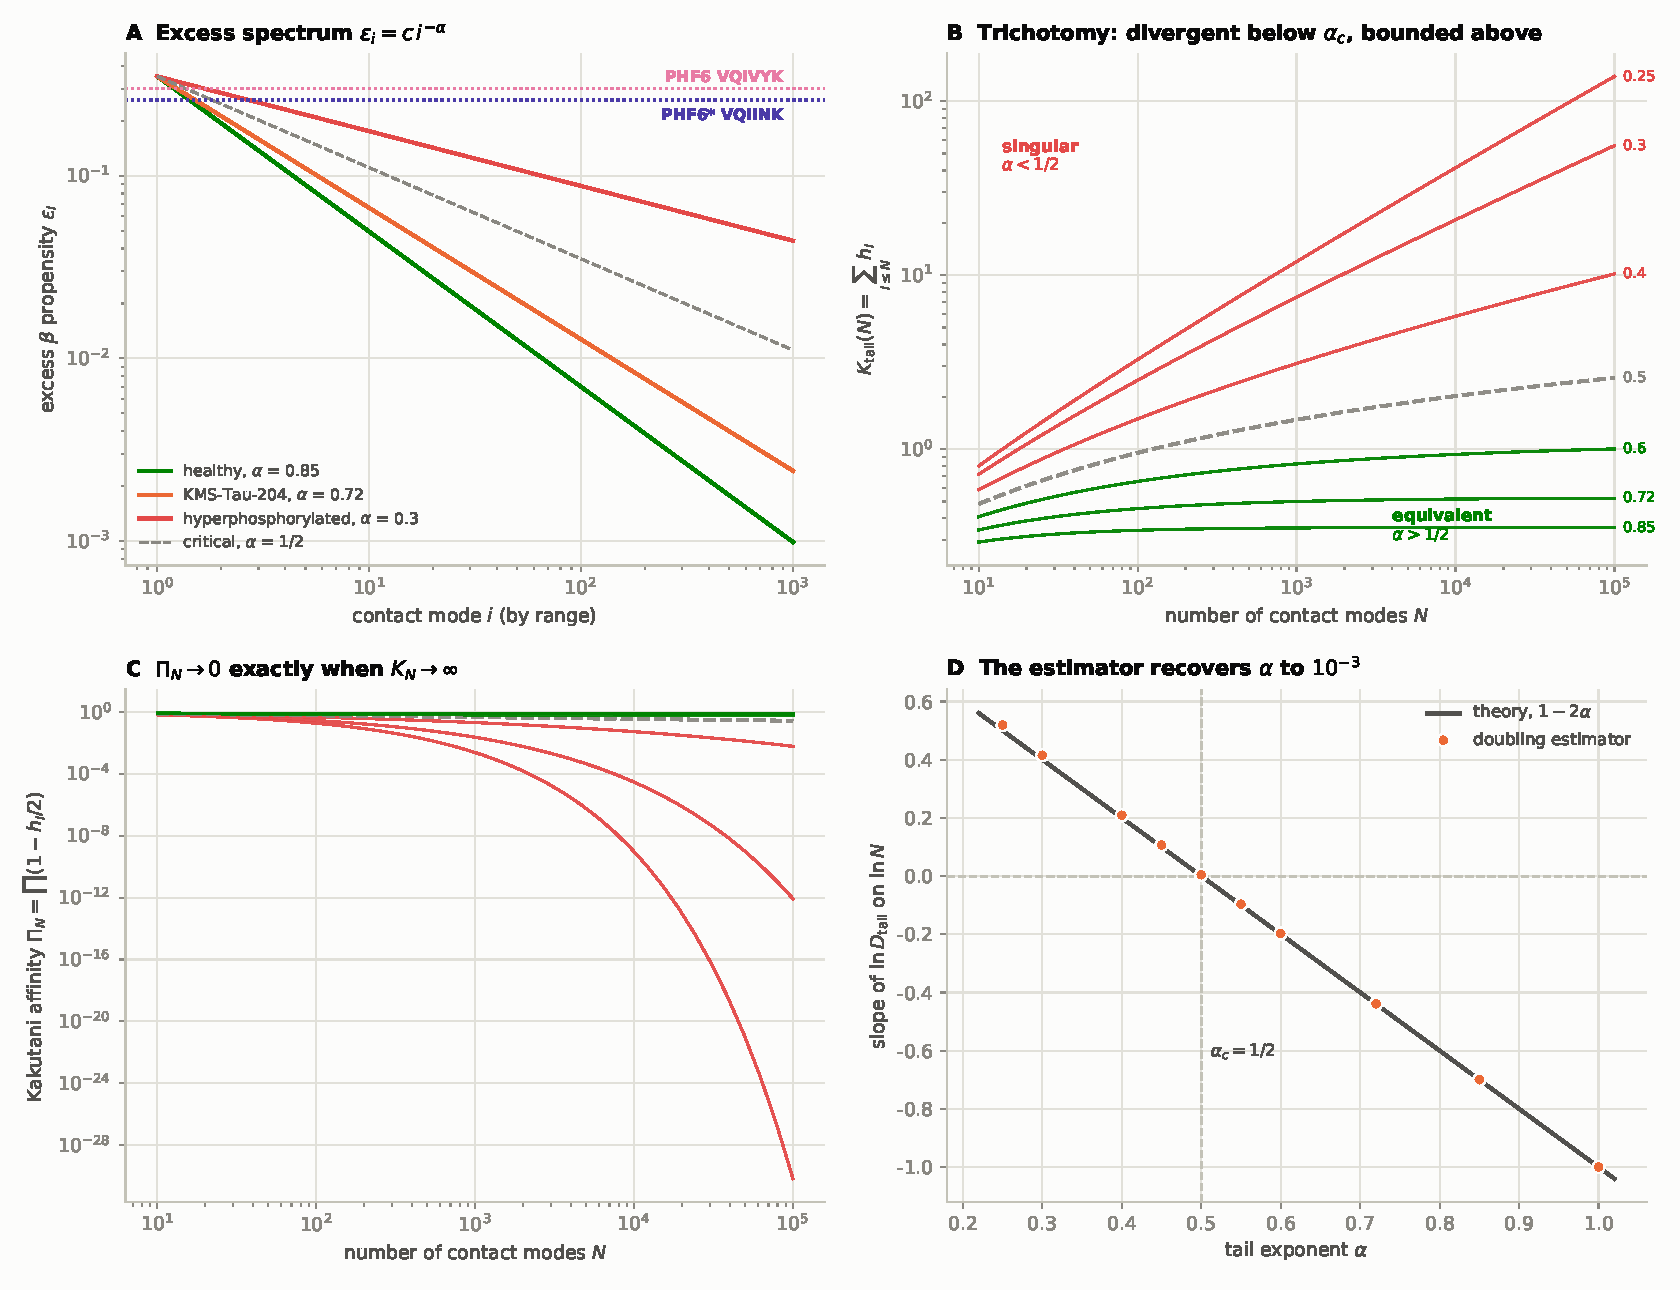
\includegraphics[width=\textwidth]{fig10_ad_tau_abeta_idp_stabilizer.pdf}
\caption{(A) The excess spectrum \eqref{eq:eps} for the three tau states, with the hot-spot levels dotted; the hexapeptide excesses are $\alpha$-independent, the tail is not. (B) The trichotomy: $\Kt(N)$ over five decades, diverging below $\ac$ (red), logarithmic at it (dashed) and bounded above (green). (C) The Kakutani affinity over the same range; $\Pi_N\to0$ exactly when $K_N\to\infty$. (D) The doubling estimator against the theoretical slope $1-2\alpha$; the residual bias at $\alpha=0.25$ is the cubic term of Proposition~\ref{prop:cubic}.}
\label{fig:main}
\end{figure}

\begin{figure}[htbp]
\centering
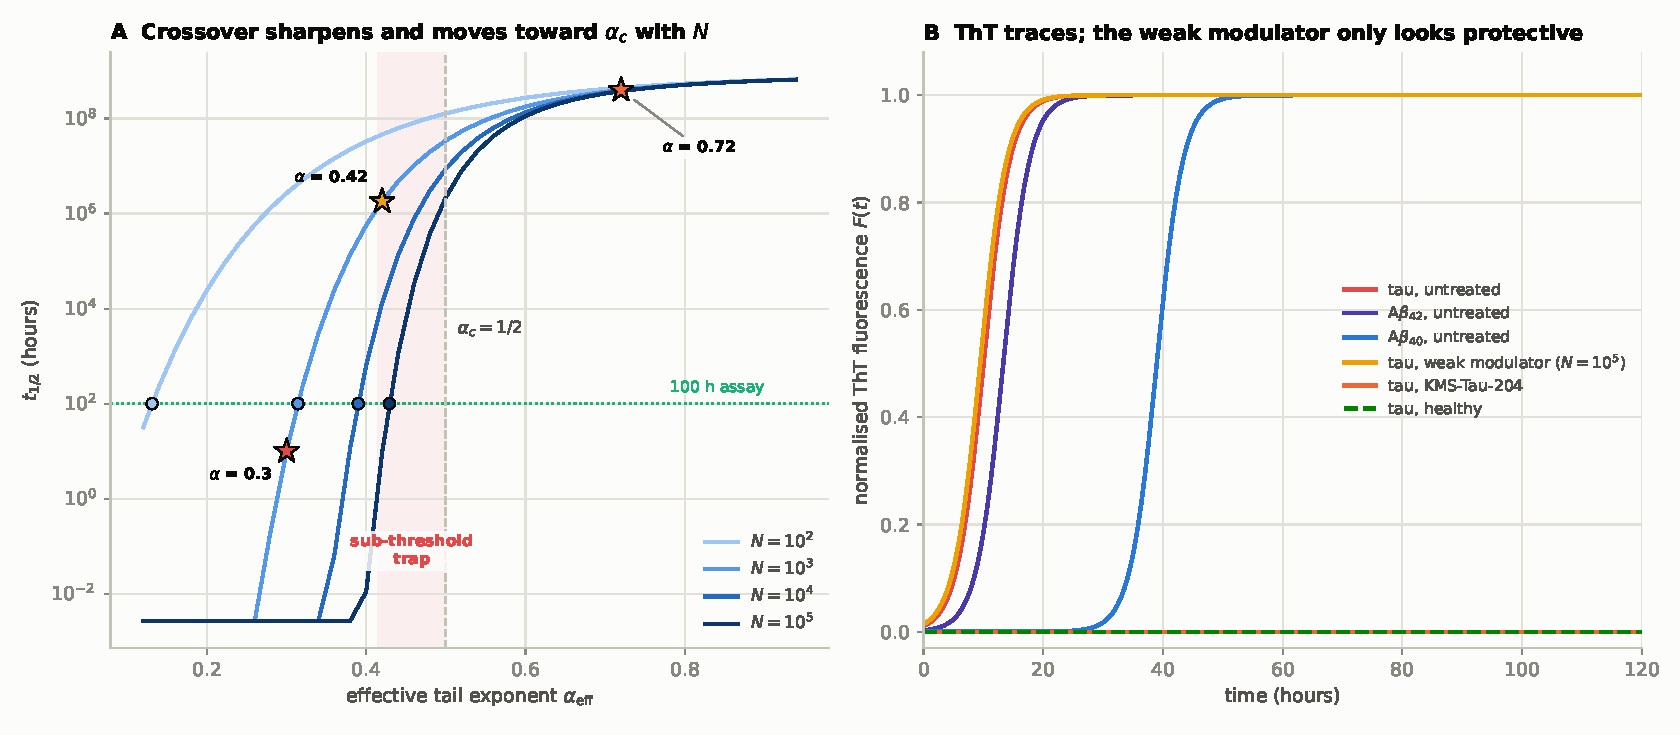
\includegraphics[width=\textwidth]{fig10b_crossover_and_tht_kinetics.pdf}
\caption{(A) Half-time against the effective tail exponent at four system sizes. The crossover sharpens and migrates toward $\ac$ as $N$ grows (Numerical observation~\ref{obs:ath}); the shaded band is the sub-threshold region in which a modulator is protected only by finite size. The three stars are the untreated ensemble, the weak modulator and \lead{}, at $N=10^3$. (B) ThT traces \eqref{eq:kinetics}. The weak modulator, evaluated at $N=10^5$, lies on top of the untreated tau trace; \lead{} and the healthy ensemble never leave zero.}
\label{fig:kinetics}
\end{figure}

\begin{table}[ht]
\centering\small\setlength{\tabcolsep}{5pt}
\caption{The three disordered segments of Definition~\ref{def:model}. The hot-spot excesses are fixed and $\alpha$-independent; $\Khot$ is the sum of their $h_i$. The tau numbering is that of the 2N4R isoform, and the ordered core of the Alzheimer filament \texttt{5O3L} begins at residue 306.}
\label{tab:peptides}
\begin{tabular}{@{}l r p{72mm} r@{}}
\toprule
segment & $n_{\mathrm{hot}}$ & hot spots & $\Khot$\\
\midrule
Tau-MTBR & $12$ & PHF6$^\ast$ \texttt{VQIINK} (275--280), $\epsilon=0.26$; PHF6 \texttt{VQIVYK} (306--311), $\epsilon=0.3$ & $1.2035$\\
$\Ab_{42}$ & $11$ & CHC \texttt{KLVFFA} (16--21), $\epsilon=0.26$; C-term \texttt{GVVIA} (38--42), $\epsilon=0.3$ & $1.0906$\\
$\Ab_{40}$ & $9$ & CHC \texttt{KLVFFA} (16--21), $\epsilon=0.26$; C-term \texttt{GVV} (38--40), $\epsilon=0.18$ & $0.6633$\\
\bottomrule
\end{tabular}
\end{table}

\begin{table}[ht]
\centering\footnotesize\setlength{\tabcolsep}{5pt}
\caption{Proposition~\ref{prop:cubic} at $p_0=0.15$, where $A_1=1.9607843$ and $B_1=5.3825452$. The last column is the measured relative remainder divided by the predicted $B_1\epsilon/A_1=2.745098\,\epsilon$. The drift at $\epsilon=10^{-1}$ is the quartic term and at $10^{-5}$ is the rounding floor of the exact value.}
\label{tab:cubic}
\begin{tabular}{@{}r r r r r r@{}}
\toprule
$\epsilon$ & $h$ exact & $A_1\epsilon^2$ & rel.\ remainder & $B_1\epsilon/A_1$ & ratio\\
\midrule
$1\times10^{-1}$ & $1.5829724 \times 10^{-2}$ & $1.9607843 \times 10^{-2}$ & $2.387 \times 10^{-1}$ & $2.745 \times 10^{-1}$ & $0.86945$\\
$1\times10^{-2}$ & $1.9091842 \times 10^{-4}$ & $1.9607843 \times 10^{-4}$ & $2.703 \times 10^{-2}$ & $2.745 \times 10^{-2}$ & $0.98458$\\
$1\times10^{-3}$ & $1.9554254 \times 10^{-6}$ & $1.9607843 \times 10^{-6}$ & $2.741 \times 10^{-3}$ & $2.745 \times 10^{-3}$ & $0.99842$\\
$1\times10^{-4}$ & $1.9602460 \times 10^{-8}$ & $1.9607843 \times 10^{-8}$ & $2.745 \times 10^{-4}$ & $2.745 \times 10^{-4}$ & $0.99984$\\
$1\times10^{-5}$ & $1.9607305 \times 10^{-10}$ & $1.9607843 \times 10^{-10}$ & $2.745 \times 10^{-5}$ & $2.745 \times 10^{-5}$ & $0.99998$\\
\bottomrule
\end{tabular}
\end{table}

\begin{table}[ht]
\centering\small\setlength{\tabcolsep}{6pt}
\caption{Proposition~\ref{prop:stable} against the textbook form \eqref{eq:index}, both compared with the two-term series of Proposition~\ref{prop:cubic}, at $p_0=0.15$. The rationalised identity converges as $\epsilon^2$ down to $\epsilon=10^{-6}$; the textbook form bottoms out near $\epsilon=10^{-4}$ and then diverges. At $\epsilon=10^{-7}$ the rationalised column rises again, for a different and unavoidable reason: $p_0+\epsilon$ is then representable only to a relative accuracy of about $10^{-10}$ in $\epsilon$ itself, so the \emph{input} limits the result. No rearrangement of the formula can pass that floor.}
\label{tab:identity}
\begin{tabular}{@{}r r r r@{}}
\toprule
$\epsilon$ & rationalised \eqref{eq:stable} & textbook \eqref{eq:index} & gain\\
\midrule
$1\times10^{-3}$ & $1.18 \times 10^{-5}$ & $1.18 \times 10^{-5}$ & $1.00 \times 10^{0}$\\
$1\times10^{-4}$ & $1.19 \times 10^{-7}$ & $1.22 \times 10^{-7}$ & $1.03 \times 10^{0}$\\
$1\times10^{-5}$ & $1.19 \times 10^{-9}$ & $5.77 \times 10^{-7}$ & $4.85 \times 10^{2}$\\
$1\times10^{-6}$ & $1.39 \times 10^{-11}$ & $4.95 \times 10^{-5}$ & $3.57 \times 10^{6}$\\
$1\times10^{-7}$ & $5.76 \times 10^{-11}$ & $7.86 \times 10^{-3}$ & $1.36 \times 10^{8}$\\
\bottomrule
\end{tabular}
\end{table}

\begin{table}[ht]
\centering\footnotesize\setlength{\tabcolsep}{4.5pt}
\caption{The trichotomy at $c=0.35$, $p_0=0.15$. $\Kt$ at four system sizes, the affinity at $N=10^5$, the measured slope of $\ln\Dt$ on $\ln N$ over $N\in[10^3,10^5]$, and the exponent recovered from it. The worst recovery error is $0.0094$, at $\alpha=0.25$ where $\epsilon_1$ is largest.}
\label{tab:trichotomy}
\begin{tabular}{@{}r r r r r r r r l@{}}
\toprule
$\alpha$ & $\Kt(10^2)$ & $\Kt(10^3)$ & $\Kt(10^4)$ & $\Kt(10^5)$ & $\Pi(10^5)$ & slope & $\widehat\alpha$ & phase\\
\midrule
$0.25$ & $3.275$ & $11.968$ & $41.436$ & $138.842$ & $6.69 \times 10^{-31}$ & $+0.5188$ & $0.2406$ & singular\\
$0.30$ & $2.489$ & $7.464$ & $20.800$ & $55.537$ & $8.53 \times 10^{-13}$ & $+0.4152$ & $0.2924$ & singular\\
$0.40$ & $1.492$ & $3.108$ & $5.804$ & $10.170$ & $6.14 \times 10^{-3}$ & $+0.2088$ & $0.3956$ & singular\\
$0.45$ & $1.182$ & $2.102$ & $3.311$ & $4.859$ & $8.75 \times 10^{-2}$ & $+0.1064$ & $0.4468$ & singular\\
$0.50$ & $0.952$ & $1.476$ & $2.019$ & $2.569$ & $2.75 \times 10^{-1}$ & $+0.0047$ & $0.4977$ & singular\\
$0.55$ & $0.781$ & $1.079$ & $1.324$ & $1.520$ & $4.66 \times 10^{-1}$ & $-0.0967$ & $0.5483$ & equivalent\\
$0.60$ & $0.652$ & $0.822$ & $0.933$ & $1.003$ & $6.03 \times 10^{-1}$ & $-0.1976$ & $0.5988$ & equivalent\\
$0.72$ & $0.455$ & $0.500$ & $0.517$ & $0.523$ & $7.67 \times 10^{-1}$ & $-0.4389$ & $0.7195$ & equivalent\\
$0.85$ & $0.342$ & $0.352$ & $0.355$ & $0.355$ & $8.34 \times 10^{-1}$ & $-0.6995$ & $0.8498$ & equivalent\\
$1.00$ & $0.271$ & $0.274$ & $0.274$ & $0.274$ & $8.69 \times 10^{-1}$ & $-0.9997$ & $0.9999$ & equivalent\\
\bottomrule
\end{tabular}
\end{table}

\begin{table}[ht]
\centering\footnotesize\setlength{\tabcolsep}{5pt}
\caption{Proposition~\ref{prop:twoterm}. The two-term formula improves on the one-term formula by about a factor ten for $c\le0.10$ and is worse at the physical $c=0.35$, where the cubic over-corrects. The two-term error falls by $9.6$ from $c=0.10$ to $c=0.03$, consistent with $O(c^2)$.}
\label{tab:twoterm}
\begin{tabular}{@{}r r r r r r r@{}}
\toprule
$\alpha$ & $c$ & $\Kt(\alpha,\infty)$ & $A\zeta(2\alpha)$ & two-term \eqref{eq:twoterm} & one-term err. & two-term err.\\
\midrule
$0.60$ & $0.35$ & $1.122973$ & $1.343076$ & $0.908702$ & $1.96 \times 10^{-1}$ & $1.91 \times 10^{-1}$\\
$0.60$ & $0.10$ & $0.101834$ & $0.109639$ & $0.099508$ & $7.66 \times 10^{-2}$ & $2.28 \times 10^{-2}$\\
$0.60$ & $0.03$ & $0.009617$ & $0.009867$ & $0.009594$ & $2.60 \times 10^{-2}$ & $2.42 \times 10^{-3}$\\
$0.72$ & $0.35$ & $0.526099$ & $0.692009$ & $0.341954$ & $3.15 \times 10^{-1}$ & $3.50 \times 10^{-1}$\\
$0.72$ & $0.10$ & $0.050362$ & $0.056491$ & $0.048326$ & $1.22 \times 10^{-1}$ & $4.04 \times 10^{-2}$\\
$0.72$ & $0.03$ & $0.004884$ & $0.005084$ & $0.004864$ & $4.09 \times 10^{-2}$ & $4.21 \times 10^{-3}$\\
$0.85$ & $0.35$ & $0.355183$ & $0.493432$ & $0.188155$ & $3.89 \times 10^{-1}$ & $4.70 \times 10^{-1}$\\
$0.85$ & $0.10$ & $0.035029$ & $0.040280$ & $0.033160$ & $1.50 \times 10^{-1}$ & $5.34 \times 10^{-2}$\\
$0.85$ & $0.03$ & $0.003452$ & $0.003625$ & $0.003433$ & $5.02 \times 10^{-2}$ & $5.51 \times 10^{-3}$\\
\bottomrule
\end{tabular}
\end{table}

\begin{table}[ht]
\centering\footnotesize\setlength{\tabcolsep}{4.5pt}
\caption{The four tau states at $N=1000$, with the critical exponent for reference. $\Khot$ is identical in every row: the stabiliser acts on the tail exponent and on nothing else, so the entire change in $t_{1/2}$ is attributable to $\alpha$.}
\label{tab:states}
\begin{tabular}{@{}l r r r r r l r r@{}}
\toprule
state & $\alpha$ & $\Khot$ & $\Kt$ & $K_N$ & $\Pi_N$ & phase & $\Delta G^{\ddagger}/\kT$ & $t_{1/2}$ (h)\\
\midrule
healthy & $0.85$ & $1.2035$ & $0.3525$ & $1.5560$ & $4.51 \times 10^{-1}$ & equivalent & $26.09$ & $5.78 \times 10^{8}$\\
\lead{} & $0.72$ & $1.2035$ & $0.5000$ & $1.7036$ & $4.18 \times 10^{-1}$ & equivalent & $25.72$ & $3.99 \times 10^{8}$\\
critical & $0.50$ & $1.2035$ & $1.4756$ & $2.6791$ & $2.56 \times 10^{-1}$ & singular & $23.27$ & $3.44 \times 10^{7}$\\
weak modulator & $0.42$ & $1.2035$ & $2.6467$ & $3.8502$ & $1.43 \times 10^{-1}$ & singular & $20.32$ & $1.81 \times 10^{6}$\\
hyperphosphorylated & $0.30$ & $1.2035$ & $7.4637$ & $8.6672$ & $1.27 \times 10^{-2}$ & singular & $8.22$ & $1.00 \times 10^{1}$\\
\bottomrule
\end{tabular}
\end{table}

\begin{table}[ht]
\centering\small\setlength{\tabcolsep}{6pt}
\caption{Section~\ref{sec:trap}: the sub-threshold false-positive trap. The weak modulator loses a factor $1.9\times10^{5}$ between a short-peptide and a full-length system size; \lead{} loses $5.8\,\%$, because above $\ac$ Proposition~\ref{prop:crossover} bounds the sum.}
\label{tab:trap}
\begin{tabular}{@{}l r r r r r r@{}}
\toprule
state & $\aeff$ & $K_N(10^3)$ & $t_{1/2}(10^3)$ & $K_N(10^5)$ & $t_{1/2}(10^5)$ & collapse\\
\midrule
hyperphosphorylated & $0.30$ & $8.6672$ & $1.00 \times 10^{1}$ & $56.7402$ & $2.70 \times 10^{-3}$ & $3.71 \times 10^{3}$\\
weak modulator & $0.42$ & $3.8502$ & $1.81 \times 10^{6}$ & $8.6897$ & $9.47 \times 10^{0}$ & $1.91 \times 10^{5}$\\
\lead{} & $0.72$ & $1.7036$ & $3.99 \times 10^{8}$ & $1.7262$ & $3.77 \times 10^{8}$ & $1.06 \times 10^{0}$\\
\bottomrule
\end{tabular}
\end{table}

\begin{table}[ht]
\centering\small\setlength{\tabcolsep}{8pt}
\caption{Numerical observation~\ref{obs:ath}: the exponent at which the half-time crosses $100$\,h, against system size. The threshold rises monotonically toward $\ac=1/2$ and stays below it. The unconditional threshold of Proposition~\ref{prop:crossover} is $\alpha^\ast=0.51789$, strictly above $\ac$.}
\label{tab:crossover}
\begin{tabular}{@{}r r@{}}
\toprule
$N$ & $\ath(N)$\\
\midrule
$10^{2}$ & $0.1311$\\
$10^{3}$ & $0.3142$\\
$10^{4}$ & $0.3899$\\
$10^{5}$ & $0.4290$\\
$10^{6}$ & $0.4524$\\
$10^{7}$ & $0.4676$\\
\bottomrule
\end{tabular}
\end{table}

\begin{table}[ht]
\centering\small\setlength{\tabcolsep}{6pt}
\caption{Section~\ref{sec:abeta}: the tail exponent $\Ab_{40}$ would need for the model to reproduce a given half-time ratio against $\Ab_{42}$, both at $\alpha=0.30$ otherwise. The first row is the hot-spot-only result, which needs no exponent difference by construction.}
\label{tab:abeta}
\begin{tabular}{@{}r r r r@{}}
\toprule
target ratio & $\alpha(\Ab_{40})$ & $\Delta\alpha$ & $t_{1/2}(\Ab_{40})$\\
\midrule
$2.93$ & $0.3000$ & $+0.0000$ & $3.90 \times 10^{1}$\,h\\
$10.00$ & $0.3073$ & $+0.0073$ & $1.33 \times 10^{2}$\,h\\
$20.00$ & $0.3117$ & $+0.0117$ & $2.66 \times 10^{2}$\,h\\
$50.00$ & $0.3179$ & $+0.0179$ & $6.66 \times 10^{2}$\,h\\
\bottomrule
\end{tabular}
\end{table}

\clearpage

%%%%%%%%%%%%%%%%%%%%%%%%%%%%%%%%%%%%%%%%%%%%%%%%%%%%%%%%%%%%%%%%%%%%%%%%%%%%%%%
\section{Assessment, limits and open problems}
\label{sec:assess}

\subsection{What was established}

\begin{table}[ht]
\centering\small\setlength{\tabcolsep}{5pt}
\caption{Status of the claims. ``Proved'' means proved here for the model of Definition~\ref{def:model}; ``numerical'' means verified computationally and not proved; ``calibrated'' means fitted to an anchor.}
\label{tab:assess}
\begin{tabular}{@{}l l l@{}}
\toprule
claim & status & evidence\\
\midrule
rationalised identity for $h$ & proved & Prop.~\ref{prop:stable}\\
gain over the textbook form & numerical & Table~\ref{tab:identity}; $3.57\times10^{6}$ at $10^{-6}$\\
cubic term at $p_0\ne1/2$ & proved & Prop.~\ref{prop:cubic}; ratio $0.99984$\\
$B_1$ odd about $1/2$, zero there & proved & Prop.~\ref{prop:cubic}\\
deviations are $O(c)$ & proved & Cor.~\ref{cor:oc}; estimator $9.4\times10^{-3}\!\to\!3.4\times10^{-4}$\\
two-term zeta formula & proved & Prop.~\ref{prop:twoterm}; error ratio $9.6$\\
series unusable at $c=0.35$ & numerical & Table~\ref{tab:twoterm}\\
estimator recovers $\alpha$ & numerical & Table~\ref{tab:trichotomy}; worst $0.0094$\\
$\Kt$ bounded above $\ac$ & proved & Prop.~\ref{prop:crossover}\\
$\alpha^\ast>\ac$ & proved & Prop.~\ref{prop:crossover}; $0.51789$\\
$\ath(N)\uparrow$, stays below $\ac$ & numerical & Obs.~\ref{obs:ath}; $0.1311\to0.4676$\\
stabiliser acts on $\alpha$ alone & by construction & Table~\ref{tab:states}; $\Khot$ constant\\
sub-threshold collapse & numerical & Table~\ref{tab:trap}; $1.91\times10^{5}$\\
barrier law and its anchor & calibrated & Eq.~\eqref{eq:kinetics}; one constant\\
\bottomrule
\end{tabular}
\end{table}

\subsection{Where this sits in the series}
Papers~I to~VI built the theory: the marginal index and its criticality theorem, the correlated index, spectral criticality, the KMS phase transition and the four-quadrant classifier, the obstruction group, and the cone geodesic. Papers~VII and~VIII turned the indices into estimators for finite trajectories and calibrated them. Paper~IX was the first application to a named target, and it used the second-order, covariance-based machinery on a folded enzyme.

This paper is the first to go back to Paper~I. That is not a step backwards: the first-order index is the right tool precisely because the target has no structure to take a covariance of, and the criticality theorem that Paper~I proved for a synthetic model is what a disordered monomer actually needs. Two things had to be added to make the transfer work, and both were forced by the biology rather than chosen: the expansion away from $p_0=1/2$, because a coil is not equally likely to be $\beta$ (Proposition~\ref{prop:cubic}); and a numerically honest evaluation of $h$, because the modes that decide the question have $\epsilon_i$ of order $10^{-3}$ and smaller (Proposition~\ref{prop:stable}). Neither would have surfaced in the symmetric, large-amplitude setting Paper~I worked in.

The one result here with no precedent in the earlier papers is Section~\ref{sec:trap}. It exists because a disordered target has a system size --- the number of contact modes --- that a folded target does not, and because that size is a property of the \emph{assay} as much as of the protein. Nothing in Papers~I to~IX has an analogue of an experiment that can be made to give the wrong answer by being made smaller.

\subsection{Limits}
We state six, in the order in which they would bite.

\textbf{(a) Contact modes are an abstraction.} There is no structure, no trajectory and no force field in this paper. The cryo-EM structures of Section~\ref{sec:cryoem} fix which segments are hot and that the monomer's long-range contacts are protective; they contribute nothing else. The index is computed exactly from a product measure, and every number is a property of Definition~\ref{def:model}.

\textbf{(b) The amplitudes are chosen, not measured.} The hot-spot excesses ($0.18$ to $0.30$), the coil baseline ($p_0=0.15$) and the tail amplitude ($c=0.35$) are inputs. What is \emph{not} an input is that the stabiliser acts on $\alpha$ alone, which is what makes Table~\ref{tab:states} a test rather than an illustration.

\textbf{(c) One constant is fitted, and everything hangs from it.} In \eqref{eq:kinetics}, $\lambda$ is set so that hyperphosphorylated tau has $t_{1/2}=10$\,h at $N=1000$. Every other half-time follows. A different anchor would move all of them together; it would not move any phase assignment, any exponent, or the collapse ratio of Table~\ref{tab:trap}, none of which depend on $\lambda$.

\textbf{(d) \lead{} is a point in parameter space, not a compound.} The model says what $\aeff$ a stabiliser must reach, and Proposition~\ref{prop:crossover} sharpens that to $\alpha^\ast=0.51789$. It does not say what molecule reaches it, and the fuzzy-binding mechanism of \cite{Heller2020} is cited as the physical precedent for the mode of action, not as a claim about any specific ligand.

\textbf{(e) Nothing here describes seeding, cross-seeding or strains.} The model is about a monomer ensemble and the barrier to forming a nucleus from it. Once a fibril exists, aggregation proceeds by elongation and secondary nucleation on the fibril surface, and those processes have nothing to do with the monomer's contact statistics. Neither does the propagation of distinct filament folds, the ``strains'' that distinguish Alzheimer tau from that of other tauopathies and which \texttt{5O3L} made visible. A compound satisfying the design law of Section~\ref{sec:pharm} would be predicted to delay primary nucleation and nothing else; in a brain that already contains seeds, that may be the wrong thing to delay. This is a limitation of scope rather than of the model, but it bears directly on what the design law is good for, and we would rather state it than let the half-times of Table~\ref{tab:states} be read as predictions about disease.

\textbf{(f) Product measures assume the contact modes are independent.} Real contacts in a disordered chain are not: excluded volume and chain connectivity correlate them. This is the most consequential simplification in the paper, because correlation changes the very exponent the argument turns on. It is the first open problem below.

\subsection{Open problems}
\begin{enumerate}[label=\textup{(\arabic*)},leftmargin=2.4em,itemsep=4pt]
\item \emph{Dependent modes.} Replace the product measure by a Markov or Gaussian-copula field over contact modes and determine how the critical exponent moves. Kakutani's theorem does not apply directly, but the Feldman--H\'aj\-ek dichotomy does for Gaussian fields, and Paper~III's spectral criticality is the natural tool. There is a reason to expect the answer to be interesting rather than merely technical: correlation between modes reduces the effective number of independent factors, and a dichotomy driven by a divergent sum over factors ought to be sensitive to that count. If the effective exponent shifts by an amount comparable to the $\Delta\alpha\approx0.018$ that Section~\ref{sec:abeta} needs, then the $\Ab_{42}$ versus $\Ab_{40}$ decomposition of Table~\ref{tab:abeta} is not safe.
\item \emph{Measuring $\alpha$.} The doubling estimator needs the excess contact probability as a function of contact order, over at least a decade of orders, for two ensembles. Paramagnetic relaxation enhancement gives distance-dependent broadening from a spin label and so reports on long-range contacts directly; single-molecule F\"orster transfer gives one contact order at a time but over a wide range of them. Neither is a measurement of $\epsilon_i$, and the gap between what they report and what the estimator consumes is the practical obstacle to using any of this. The concrete question is: what is the smallest set of labelling positions whose pairwise statistics, measured for a treated and an untreated ensemble, would place the pair on the correct side of $\ac$ with useful confidence? A negative answer would be almost as valuable as a positive one, because it would say the design law is not measurable as stated.
\item \emph{Testing the trap.} Take one aggregation inhibitor with a published effect on a hexapeptide or short construct, and run it against constructs of systematically increasing length under otherwise identical conditions. The model predicts something quite specific: a compound whose protection is finite-size should lose it monotonically and without a threshold, since $\ath(N)$ rises smoothly; a compound above $\alpha^\ast$ should show a half-time that is flat in construct length. The two behaviours are distinguishable with three or four constructs, and the experiment needs no new chemistry. If the collapse is not seen, the trap is an artefact of the product-measure assumption and the model is wrong in an interesting way.
\item \emph{The barrier law.} Equation~\eqref{eq:kinetics} is phenomenological. Derive the dependence of the nucleation barrier on the Kakutani separation from a first-passage argument, rather than positing linearity and fitting one constant.
\item \emph{The quartic coefficient.} Proposition~\ref{prop:cubic} stops at the cubic term. The quartic coefficient at general $p_0$ would give the next correction in Proposition~\ref{prop:twoterm} and, with it, a usable series at the physical amplitude $c=0.35$, which is currently out of reach.
\end{enumerate}

\subsection*{Data and code availability}
Everything in this paper is produced by two scripts in \texttt{code/}:
\begin{itemize}[leftmargin=1.6em,itemsep=2pt]
\item \texttt{exp10\_ad\_tau\_abeta\_idp\_stabilizer.py}, the experiment;
\item \texttt{exp10\_lib.py}, its model library;
\item \texttt{paper10\_compute\_tables.py}, the companion that writes the table bodies.
\end{itemize}
The five data files are in \texttt{data/}, the two figures in \texttt{figures/} and the logs in \texttt{results/}. Seventeen model unit tests and the twelve inherited tests of \pkg{} pass.

\subsection*{Funding}
This project was supported by the National Natural Science Foundation of China (No.~22464010), the Guangxi Natural Science Foundation of China (No.~2025GXNSFAA069294), and the 2025 Bagui Youth Top Talent Project.

%%%%%%%%%%%%%%%%%%%%%%%%%%%%%%%%%%%%%%%%%%%%%%%%%%%%%%%%%%%%%%%%%%%%%%%%%%%%%%%
\begin{thebibliography}{99}
\bibitem{Chen2026} R.~Chen, \emph{Localized Bost--Connes systems}, monograph, 2026, DOI 10.5281/zenodo.22883179.
\bibitem{ChenChen2026I} Z.~Chen and R.~Chen, \emph{Statistical pharmacology via Kakutani dichotomy I: the marginal drug Kakutani index and the $\alpha_c=1/2$ criticality theorem in high-dimensional conformational ensembles}, 2026, DOI 10.5281/zenodo.23005921 (version 1.1: 10.5281/zenodo.23018827).
\bibitem{ChenChen2026II} Z.~Chen and R.~Chen, \emph{Statistical pharmacology via Kakutani dichotomy II: the correlated Kakutani index, the 99.95\% covariance dominance theorem, and spectral fingerprints of cryptic allostery}, 2026, DOI 10.5281/zenodo.23012217.
\bibitem{ChenChen2026III} Z.~Chen and R.~Chen, \emph{Statistical pharmacology via Kakutani dichotomy III: spectral Kakutani--Feldman--H\'ajek criticality of correlated conformational modes}, 2026, DOI 10.5281/zenodo.23015709.
\bibitem{ChenChen2026IV} Z.~Chen and R.~Chen, \emph{Statistical pharmacology via Kakutani dichotomy IV: KMS inverse-temperature criticality $\beta_c=1$, pocket-to-distal tail allostery, and the four-quadrant ligand classification}, 2026, DOI 10.5281/zenodo.23018236.
\bibitem{ChenChen2026V} Z.~Chen and R.~Chen, \emph{Statistical pharmacology via Kakutani dichotomy V: the chemical obstruction group, Borel--Cantelli tail order parameters, and the relative-entropy staircase}, 2026, DOI 10.5281/zenodo.23027704.
\bibitem{ChenChen2026VI} Z.~Chen and R.~Chen, \emph{Statistical pharmacology via Kakutani dichotomy VI: Wasserstein phase separation, the single-step scan barrier, and cone-geodesic collective moves}, 2026, DOI 10.5281/zenodo.23029360.
\bibitem{ChenChen2026VII} Z.~Chen and R.~Chen, \emph{Statistical pharmacology via Kakutani dichotomy VII: the kakutani\_pharma pipeline, Ledoit--Wolf regularized CKI, split-trajectory null subtraction, and shell-scaling exponents in multi-domain allostery}, 2026, DOI 10.5281/zenodo.23039869.
\bibitem{ChenChen2026VIII} Z.~Chen and R.~Chen, \emph{Statistical pharmacology via Kakutani dichotomy VIII: empirical validation on experimental all-atom protein ensembles, influence-function block selection, and bootstrap coverage calibration}, 2026, DOI 10.5281/zenodo.23045772.
\bibitem{ChenChen2026IX} Z.~Chen and R.~Chen, \emph{Statistical pharmacology via Kakutani dichotomy IX: Notch-sparing gamma-secretase modulators for Alzheimer's disease, Schur-complement confinement of the catalytic block, and a cone-geodesic model of processive trimming}, 2026, DOI 10.5281/zenodo.23051518.
\bibitem{ChenChen2026S} Z.~Chen and R.~Chen, \emph{Kakutani--KMS theory of ligand-induced conformational phase transitions}, 2026, DOI 10.5281/zenodo.23042828.
\bibitem{Fitzpatrick2017} A.~W.~P. Fitzpatrick, B.~Falcon, S.~He, A.~G. Murzin, G.~Murshudov, H.~J. Garringer, R.~A. Crowther, B.~Ghetti, M.~Goedert and S.~H.~W. Scheres, \emph{Cryo-EM structures of tau filaments from Alzheimer's disease}, Nature \textbf{547} (2017), 185--190. PDB \texttt{5O3L}.
\bibitem{Gremer2017} L.~Gremer, D.~Sch\"olzel, C.~Schenk, E.~Reinartz, J.~Labahn, R.~B.~G. Ravelli, M.~Tusche, C.~Lopez-Iglesias, W.~Hoyer, H.~Heise, D.~Willbold and G.~F. Schr\"oder, \emph{Fibril structure of amyloid-$\beta$(1--42) by cryo-electron microscopy}, Science \textbf{358} (2017), 116--119. PDB \texttt{5OQV}.
\bibitem{Heller2020} G.~T. Heller, F.~A. Aprile, T.~C.~T. Michaels, R.~Limbocker, M.~Perni, F.~S. Ruggeri, B.~Mannini, T.~L\"ohr, M.~Bonomi, C.~Camilloni, A.~De~Simone, I.~C. Felli, R.~Pierattelli, T.~P.~J. Knowles, C.~M. Dobson and M.~Vendruscolo, \emph{Small-molecule sequestration of amyloid-$\beta$ as a drug discovery strategy for Alzheimer's disease}, Sci. Adv. \textbf{6} (2020), eabb5924.
\bibitem{Jeganathan2006} S.~Jeganathan, M.~von~Bergen, H.~Brutlach, H.-J. Steinhoff and E.~Mandelkow, \emph{Global hairpin folding of tau in solution}, Biochemistry \textbf{45} (2006), 2283--2293.
\bibitem{Kakutani1948} S.~Kakutani, \emph{On equivalence of infinite product measures}, Ann. of Math. \textbf{49} (1948), 214--224.
\bibitem{Takami2009} M.~Takami, Y.~Nagashima, Y.~Sano, S.~Ishihara, M.~Morishima-Kawashima, S.~Funamoto and Y.~Ihara, \emph{$\gamma$-Secretase: successive tripeptide and tetrapeptide release from the transmembrane domain of $\beta$-carboxyl terminal fragment}, J. Neurosci. \textbf{29} (2009), 13042--13052.
\bibitem{vonBergen2000} M.~von~Bergen, P.~Friedhoff, J.~Biernat, J.~Heberle, E.-M. Mandelkow and E.~Mandelkow, \emph{Assembly of $\tau$ protein into Alzheimer paired helical filaments depends on a local sequence motif ($^{306}$VQIVYK$^{311}$) forming $\beta$ structure}, Proc. Natl. Acad. Sci. USA \textbf{97} (2000), 5129--5134.
\end{thebibliography}

\end{document}
